

\documentclass{article}

\usepackage{multicol}
\setlength{\columnsep}{1.2cm}
\usepackage{pgfplots}
\pgfplotsset{compat = newest}
\usepackage{titlesec}
\usepackage{graphicx}
\usepackage{wrapfig}
\usepackage{amsfonts}
\usepackage{tikz}
\usepackage{amssymb}
\usepackage{amsfonts}
\usepackage{amsmath}


\title{Intro to Functions}
\author{Anna Denisova}
\date{2023}

\begin{document}

\maketitle
\tableofcontents

%----------------------------------------------------------

\newpage
\section{Function Definitions}

%----------------------------------------------------------

\newpage
\section{Function Notation}

%----------------------------------------------------------

\newpage
\section{Parent Functions}

%----------------------------------------------------------

\newpage
\section{Domain and Range}


%----------------------------------------------------------

\newpage
\section{The Inverse Function}


%----------------------------------------------------------

\newpage
\section{Transformations}

\subsection{$f(x) = -2\sqrt{x-3} + 5$}
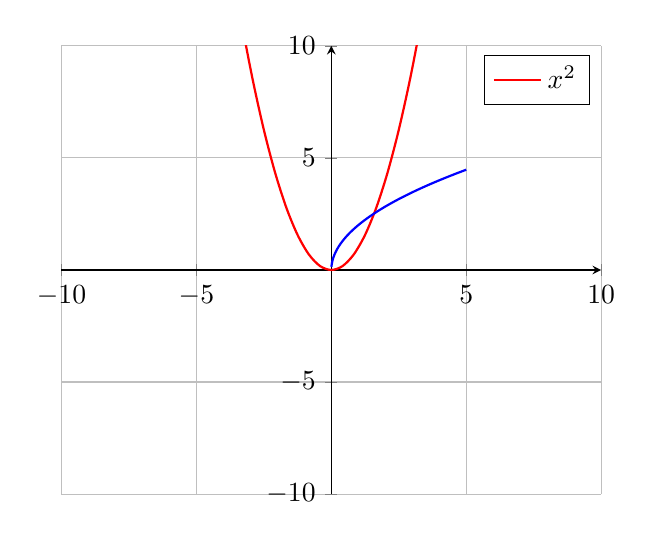
\begin{tikzpicture}
    \begin{axis}[
        xmin = -10, xmax = 10,
        ymin = -10, ymax = 10,
        grid = both,
        major grid style = {lightgray},
        minor grid style = {lightgray!25},
        axis lines = center
        ]
        \addplot[thick, smooth, red]{x^2};
        \addplot[thick, smooth, blue, samples = 1000]{2*sqrt(x)};

        \legend{
            $x^2$,
        }

    \end{axis}
\end{tikzpicture}
    

%----------------------------------------------------------

\newpage
\section*{Piecewise Functions}

\[ \begin{cases} 
    function & restrictions \\
    x & 0 < x\leq 100 \\
    1 & 100 < x 
 \end{cases}
\]


%----------------------------------------------------------

\end{document}